\documentclass[14pt]{extreport}
\usepackage{gost}
\usepackage{hyperref}
\usepackage{makecell}
\usepackage{ragged2e}
\usepackage{graphicx}%Вставка картинок правильная
\usepackage{float}%"Плавающие" картинки
\usepackage{wrapfig}%Обтекание фигур (таблиц, картинок и прочего)
	
\usepackage{lscape}
\justifying
\makeatletter
\@addtoreset{figure}{part}% Reset figure numbering at every part
\makeatother
\renewcommand{\thefigure}{\arabic{figure}}% Figure number is part.figure
\renewcommand{\thetable}{\arabic{table}}



%Тут можно вставить дополнительные пакеты

\begin{document}
\pagestyle{empty} %  выключаем нумерацию
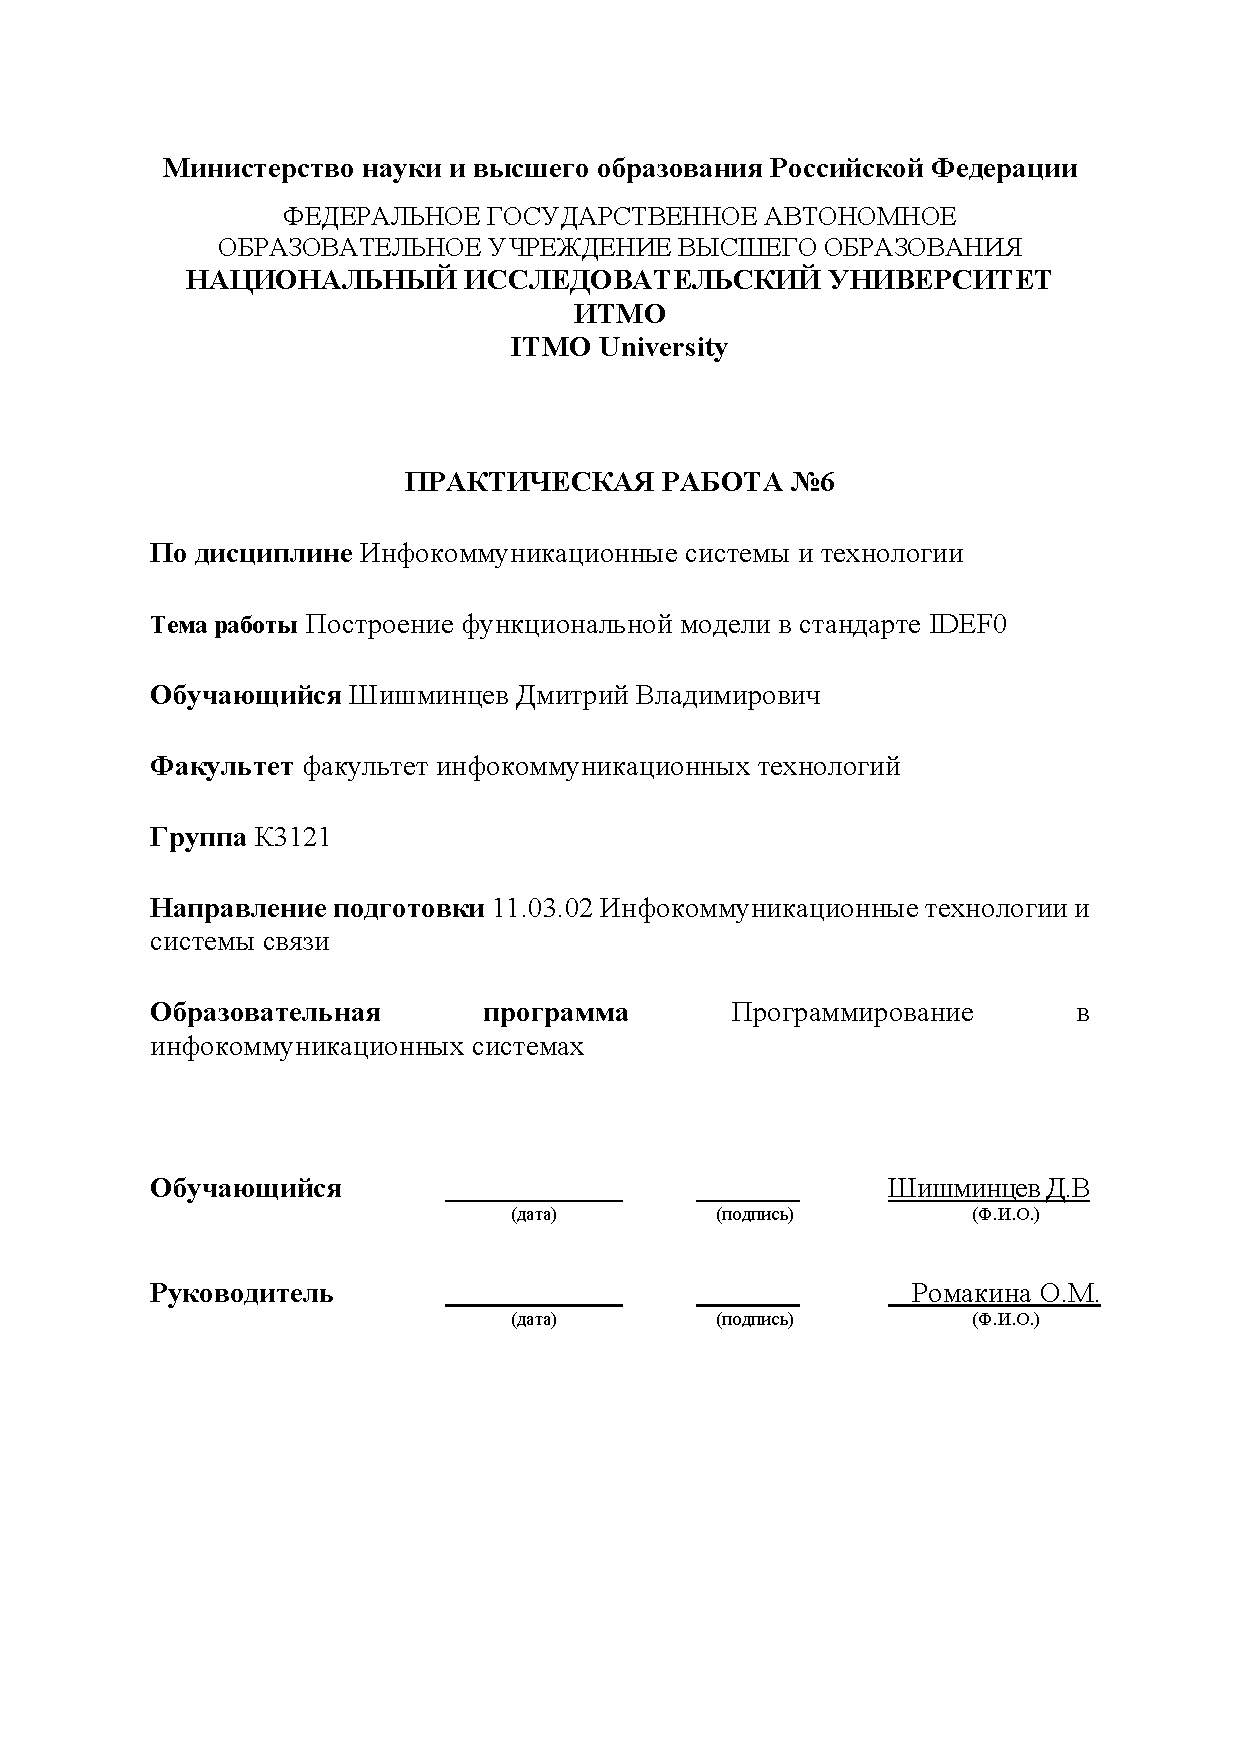
\includepdf[pages=-,pagecommand={}]{title_page.pdf}


\pagestyle{plain} % включаем нумерацию
\tableofcontents
\intro\label{intro} 

Данная практическая работа содержит в себе краткое описание предметной области функционирования и основных пользователей будующей информационной системы, так же была разработана функциональная модель информационной системы в стандарте IDEF0.


\chapter{ОПИСАНИЕ ИДЕИ ИНФОРМАЦИОННОЙ СИСТЕМЫ \label{chapter1}}

\section{Основной функционал}

Информационная система MEET ME представляет из себя веб-приложение для планирования встреч с друзьями и родственниками в виде календаря. 
Приложение показывает пересечение свободного времени пользователя с одним или несколькими его друзьями.
C помощью данного приложения пользователь может эффективно планировать встречи со своими друзьями, родственниками или знакомыми не тратя огромное количество времени на согласования времени. 

После создания аккаунта, пользователю будет предложено настроить свое расписание. Пользователь выбирает дни и время, когда он имеет возможность для встречи. 
Настроив свое расписание, пользователь должен добавить своих друзей.  Добавление друзей идет посредством отправки запроса другу на его электронную почту указаную при регистрации аккаунта.

Настроив свое расписание и добавив друзей, пользователю начинают отображаться пересечения в расписании с его друзьями в виде календаря. Пользователю не показывается полностью расписание встреч его друзей ради сохранения приватности. Пользователь может отправить приглашение на встречу своему другу если их свободное время пересекается в приложении. Приглашение отобразится у его друга и он сможет принять или отклонить его. Приняв приглашение у обоих пользователей отобразится встреча в их календаре. 

\section{Основные пользователи}

Информационная система будет иметь только прямых конечных пользователей. Система не требует модераторов, менеджеров и прочих пользователей.
Целевая аудитория данной информационной системы достаточно широка. Основными пользователями будут молодые, общительные люди, которые стараются грамотно распределять свое время (ученики старших классов, студенты, работающая молодежь).


\chapter{Функциональные модели}

\section{Функциональные модели по стандарту IDEF0}
В данном разделе представлены функциональные модели по стандарту IDEF0. Изучив стандарт IDEF0 (учебное пособие \ref{bib:bib1}), была разработана контекстная диаграмма (рисунок \ref{fig:d1}), декомпозиция контекстной диаграммы (рисунок \ref{fig:d2}),  декомпозиция блока <<Авторизация>> (рисунок \ref{fig:d3}), декомпозиция блока <<Определение общего свободного времени>> (рисунок \ref{fig:d4}), декомпозиция блока <<Определение расписания пользователя>> (рисунок \ref{fig:d5}).
\begin{landscape}
    \begin{figure}[h]   
        \centering
        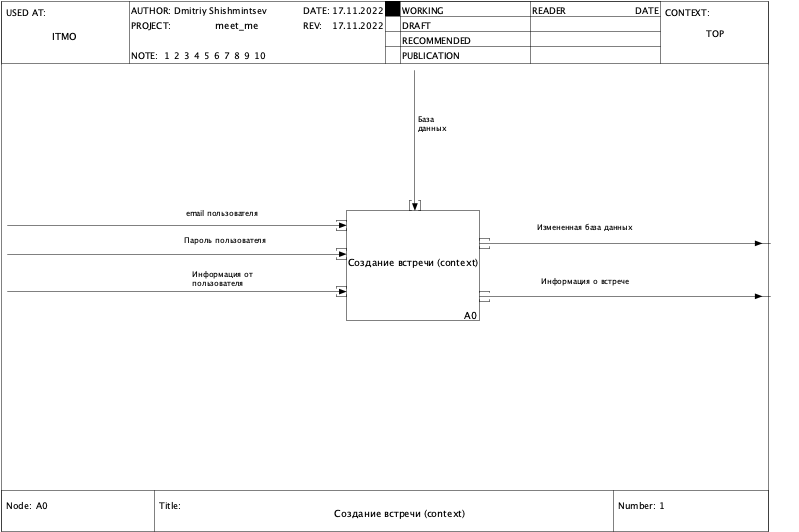
\includegraphics[width=1\linewidth]{img/01_A0.png}
        \caption{ Контекстная диаграмма}
        \label{fig:d1}
    \end{figure}
    \begin{figure}[h]   
        \centering
        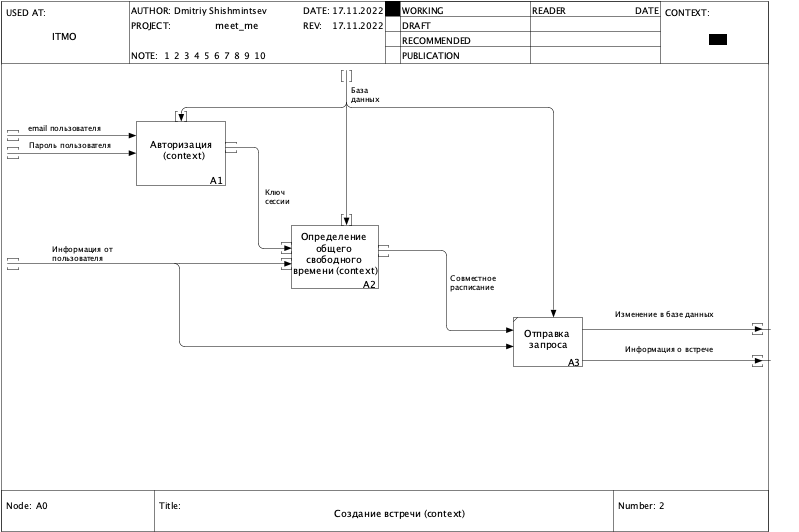
\includegraphics[width=1\linewidth]{img/02_A0.png}
        \caption{ Декомпозиция контекстной диаграммы}
        \label{fig:d2}
    \end{figure}
    \begin{figure}[h]   
        \centering
        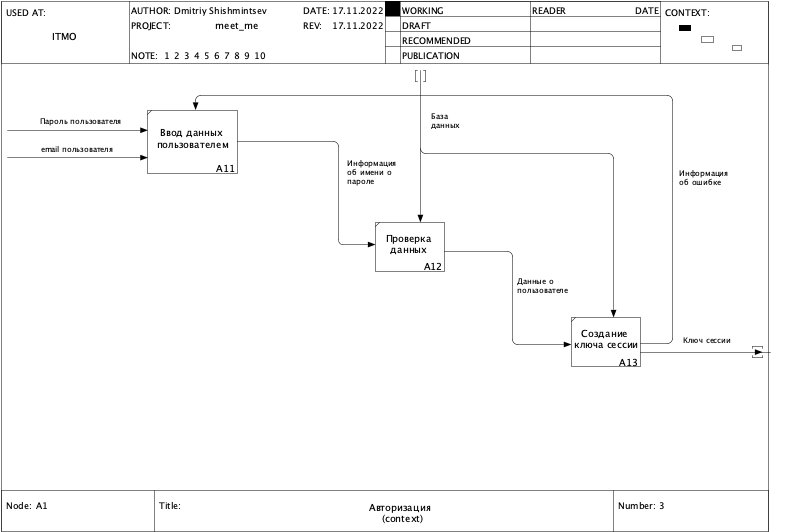
\includegraphics[width=1\linewidth]{img/03_A1.png}
        \caption{ Декомпозиция блока <<Авторизация>>}
        \label{fig:d3}
    \end{figure}
    \begin{figure}[h]   
        \centering
        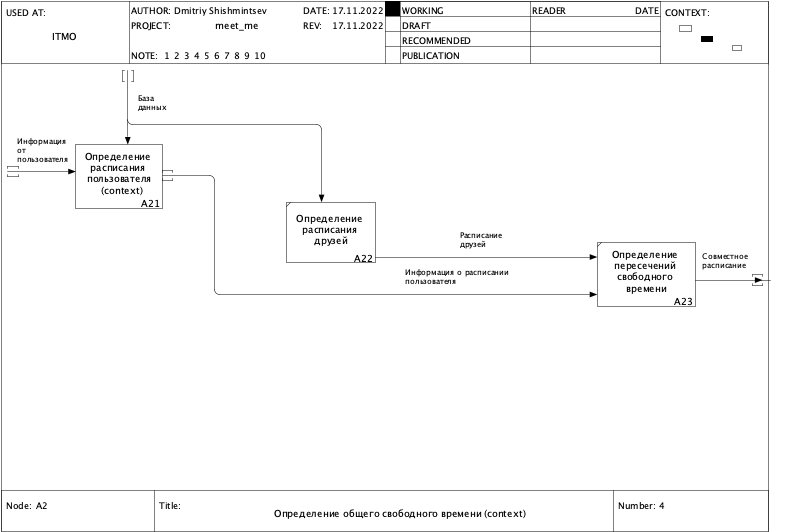
\includegraphics[width=1\linewidth]{img/04_A2.png}
        \caption{ Декомпозиция блока <<Определение общего свободного времени>>}
        \label{fig:d4}
    \end{figure}
    \begin{figure}[h]   
        \centering
        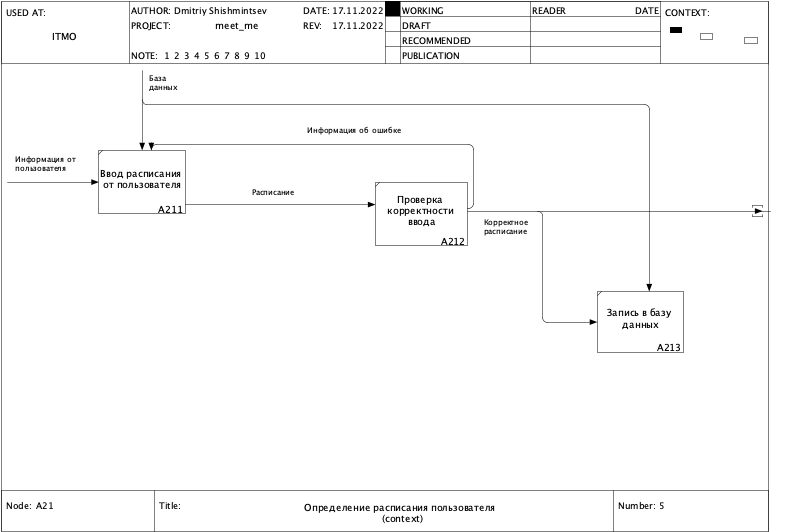
\includegraphics[width=1\linewidth]{img/05_A21.png}
        \caption{ Декомпозиция блока <<Определение расписания пользователя>>}
        \label{fig:d5}
    \end{figure}
    
\end{landscape}

\conclusions

Был составлен отчет, кратко описана основная предметная область функционирования будующей информационной системы, разработаны функциональные модели будующей информационной системы согласно стандарту IDEF0.

\newpage
\begin{thebibliography}{99}
	\bibitem{bib1} 	\label{bib:bib1} В. И. Горбаченко. <<СОЗДАНИЕ ФУНКЦИОНАЛЬНОЙ МОДЕЛИ ИНФОРМАЦИОННОЙ СИСТЕМЫ С ПОМОЩЬЮ CASE-средства CA ERwin Process Modeler 7.3>> - Пенза 2010 - 25-55с.
\end{thebibliography}

\end{document}
